\section{Failure Case: en-fr on the Loose-Filter v2 Corpus}
\label{sec:enfr_v2}

This section reports the failure side of the 2x2 ablation. Base v2 and Big v2 share the pipeline, SPM, eval, and hyperparameters of their v1.1 counterparts; only the training corpus changes (v1's 9.3M strict-filter $\rightarrow$ v2's 30M loose-filter, drawn from the same WMT14 source pool). Both v2 runs converge cleanly. \emph{Both land below their v1 counterparts}, and \emph{Big v2 lands below Base v2} on identical data. The 2x2 closes here.

\subsection{Corpus construction}
v2 starts from the same WMT14 en-fr raw $\sim$~40.8M, cleaned with the same per-pair filters as v1, but \emph{without} the 10M-head cap. 30.1M pairs survive (74\% keep rate, vs.\ v1's 93\% on the head 10M). The 19-point keep-rate gap quantifies how much noisier the long tail is once the cap is removed.

A schedule re-tune is required because v2 is $3.2\times$ larger: Base v2 runs 600K steps (vs.\ Base v1.1's 122K) and Big v2 runs 800K (vs.\ Big v1.1's 280K), preserving the $\sim$~3-epoch budget. Warmup is scaled proportionally (4K~$\rightarrow$~12K for Base, 8K~$\rightarrow$~24K for Big). All other hyperparameters are unchanged.

\subsection{Base v2: 60M parameters, 30M loose data}
\label{sec:base_v2}
Trained for 600K steps (4 epochs over 30M); best converged valid is 28.66, and averaging 5 checkpoints gives valid 29.23 / test 33.90. Total wall-clock: $\sim$~14~h.

This sits \textbf{below Base v1.1} on both splits: $-1.29$ valid, $-1.41$ test. Despite seeing $3.2\times$ more data and running $4.9\times$ more optimizer steps, v2 underperforms v1.1 by more than a full BLEU.

\begin{figure}[t]
\centering
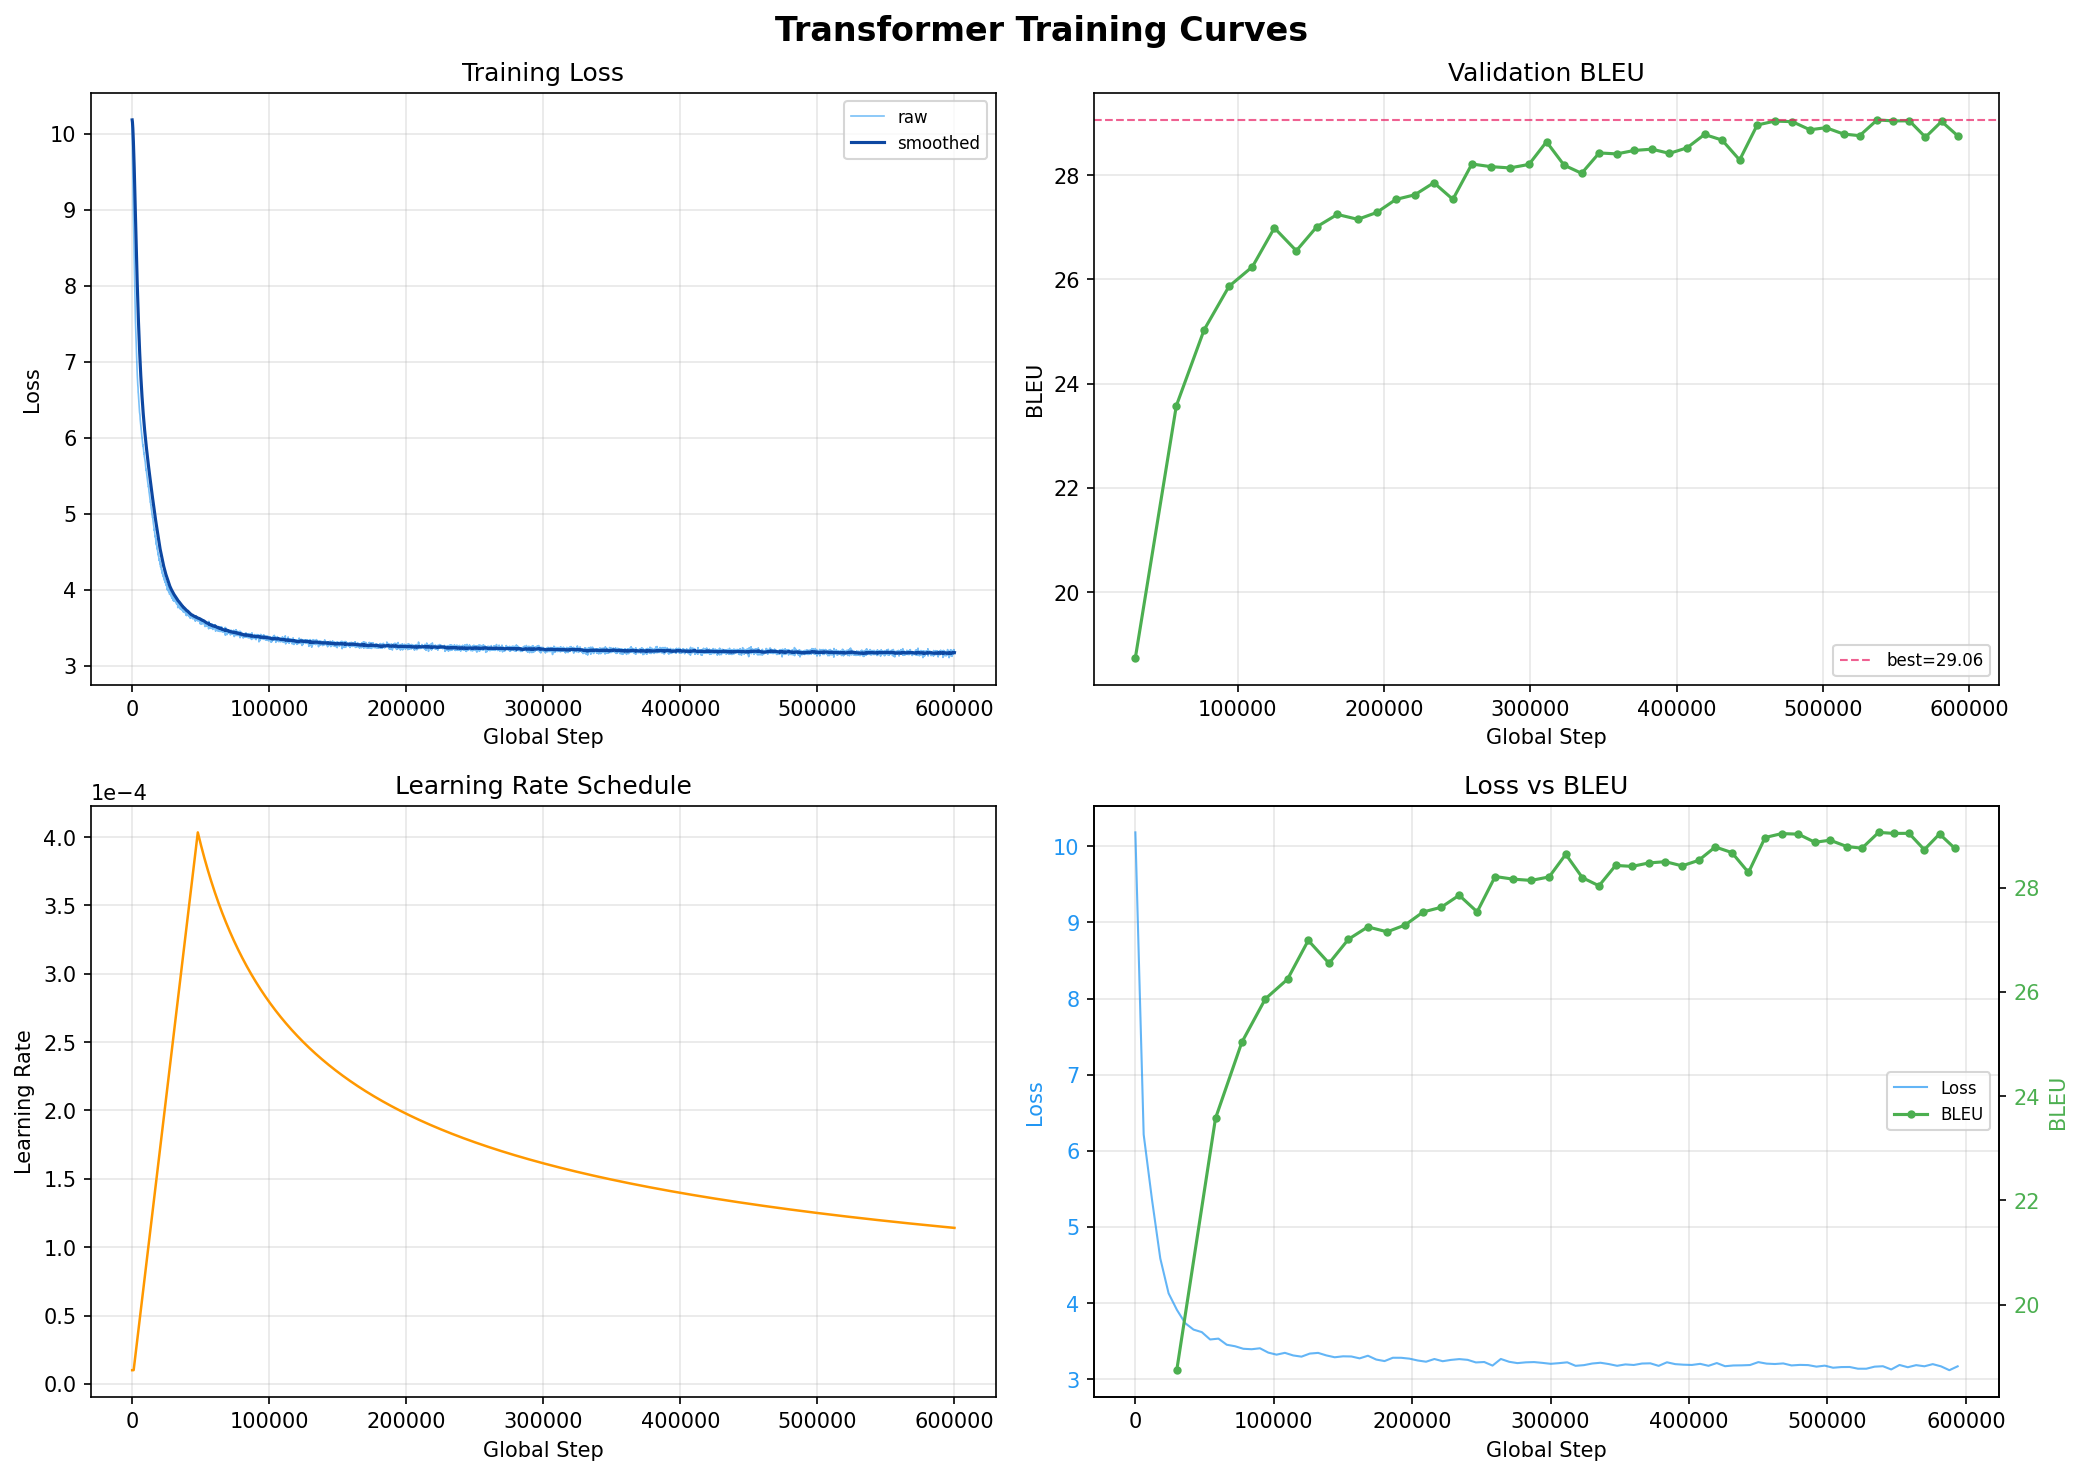
\includegraphics[width=\columnwidth]{figures/base_v2_curves.png}
\caption{Base v2 training curves (60M parameters, 600K steps, 30M loose-filter en-fr corpus). Loss converges smoothly; BLEU plateaus near 28.5--29 from step 400K onwards, $\sim$~1.4 below Base v1.1's averaged 30.52 baseline despite $4.9\times$ the optimizer steps and $3.2\times$ the data.}
\label{fig:base_v2_curves}
\end{figure}

\subsection{Big v2: 209M parameters, 30M loose data}
\label{sec:big_v2}
Trained from scratch for 800K planned steps; halted at 416K once valid BLEU plateaued and a single eval dipped below the running best. Best single-checkpoint valid is 27.77; averaging 5 checkpoints in [345K, 416K] gives valid 28.91 / test 33.03. Total wall-clock: $\sim$~9~h to halt.

This sits \textbf{below Base v2} on both splits: $-0.32$ valid, $-0.87$ test. The same $3.5\times$ extra parameters that paid $+0.56$ on v1 (\S\ref{sec:v1_capacity}) cost $-0.87$ here. The capacity gap has flipped sign.

\subsection{The 2x2 result}
\label{sec:two_by_two}

\begin{table}[t]
\centering
\small
\begin{tabular}{lrrr}
\toprule
\textbf{Data} & \textbf{Base (60M)} & \textbf{Big (209M)} & \textbf{$\Delta$} \\
\midrule
v1.1 (9.3M strict) & 35.31 & \textbf{35.87} & $\mathbf{+0.56}$ \\
v2 (30M loose)     & \textbf{33.90} & 33.03 & $\mathbf{-0.87}$ \\
\midrule
\textbf{Quality drop} & $-1.41$ & $-2.84$ & --- \\
\bottomrule
\end{tabular}
\caption{The 2x2 result: test BLEU on newstest2014; sacrebleu 13a, beam=5, length-penalty=1.0, 5-checkpoint averaged. Bold marks the better model within each row (capacity gap) and column (data-quality gap). The Big$-$Base difference flips sign: $+0.56$ on clean data, $-0.87$ on noisy data. Equivalently, the v1$\rightarrow$v2 quality drop is twice as large for Big ($-2.84$) as for Base ($-1.41$).}
\label{tab:two_by_two}
\end{table}

Table~\ref{tab:two_by_two} is the central empirical claim of the paper. Two ways to read it:
\begin{enumerate}
\item \textbf{Row-wise (capacity gap):} on clean data Big beats Base by $+0.56$; on noisy data Big falls below Base by $-0.87$. A single architectural change has opposite effects on opposite-quality data.
\item \textbf{Column-wise (data-quality drop):} both models lose BLEU on the noisier corpus, but Big loses twice as much ($-2.84$ vs.\ $-1.41$). Capacity does not absorb noise; it amplifies its cost.
\end{enumerate}

These are the same claim viewed two ways: capacity is a force multiplier whose sign depends on the supervision signal it is multiplying.

\subsection{Why v2 is noisy: direct evidence}
We attribute v2's degradation to noise in the extra 20M pairs beyond the v1 head 10M. Three pieces of supporting evidence:

\paragraph{Spike-guard activations.} The loss-spike guard (\S\ref{sec:setup}) fires when a batch's loss exceeds $1.3\times$ the EMA --- intended to drop pathologically wrong batches. On Base v1.1's 122K-step run it fires \textbf{0 times}; on Big v2's 416K-step run it fires \textbf{12 times} ($\approx$~1 per 35K steps). The 0-vs-nonzero contrast is the direct signal: clean v1 contains no batches that loss-spike a competent model, while v2 contains 12 such batches over its longer run. \S\ref{sec:methodology} adds a methodology caveat about cross-capacity spike-guard comparisons.

\paragraph{Sample inspection.} Manual inspection of the 100 lowest-scoring v2 pairs by CometKiwi-22 (``low'' in the 0.05--0.3 range) reveals the expected pathologies: source sentences echoed verbatim as ``translation'', misaligned pairs, repeated boilerplate from web-scraped UN documents, partial translations, and reverse-direction translations (fr~$\rightarrow$~en where en~$\rightarrow$~fr was expected). These pairs survive the per-pair length and ratio filters because those filters are token-counting heuristics and do not detect semantic misalignment.

\paragraph{Schedule was not the cause.} An earlier v2 attempt with 200K steps (a linear $2\times$ over v1's 100K) underfit badly --- training loss had not reached its v1 floor by the schedule end. We rejected that attempt and adopted 600K (a $4\times$ schedule for $3.2\times$ data, with proportional warmup), which trains to a tight loss floor. The headline 600K-step Base v2 result is post-convergence, not under-training.

\subsection{Big v2 was halted early: was that the right call?}
Big v2 was planned for 800K steps and halted at 416K. The halt rule: a single eval drops below the running best, AND the run has been pathologically slow to find new bests. At halt, Big v2's averaged BLEU was 33.03 / 28.91, already well below Base v2's 33.90 / 29.23 at the same wall-clock.

Could continued training to 800K have lifted Big v2 above Base v2? The trajectory in Figure~\ref{fig:big_v2_curves} makes this unlikely under the observed trend: late-training BLEU oscillates within $\pm 0.5$ around 27.7--28.0 from step 300K through 416K with no upward drift, while training loss plateaus at $\sim$~3.0. Further steps would have kept reducing loss on noisy patterns; we have no evidence they would have produced additional BLEU gain. We accept the halt as the conservative call and note that continued training could plausibly drift Big v2 further below 33.03 (more noise fitting) rather than above.

\begin{figure}[t]
\centering
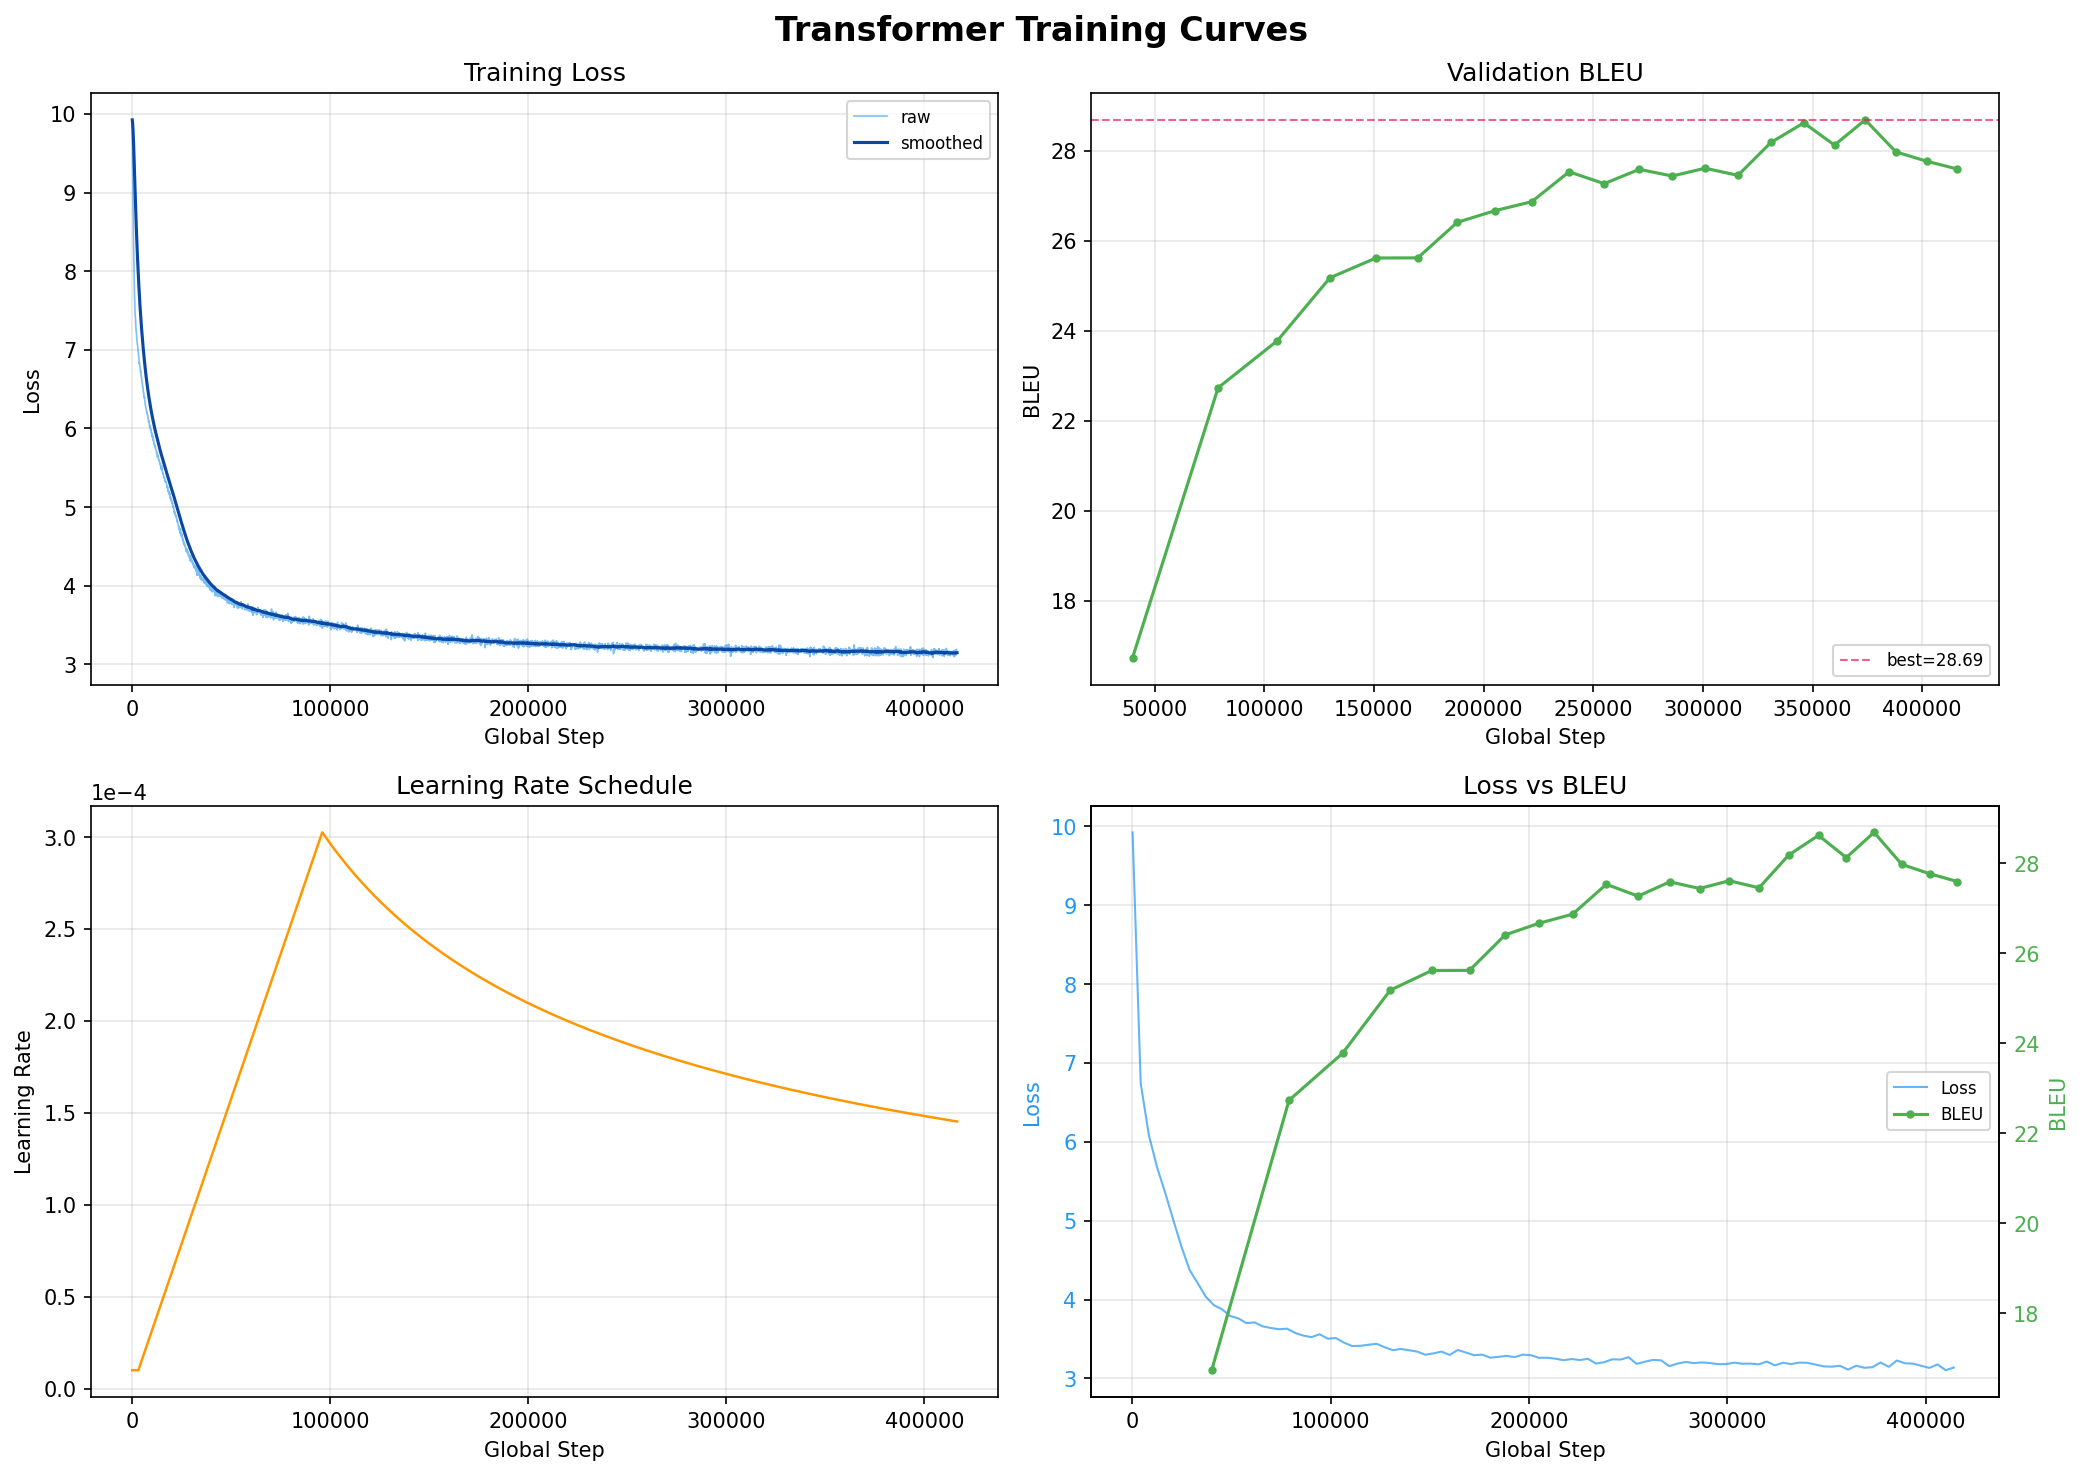
\includegraphics[width=\columnwidth]{figures/big_v2_curves.png}
\caption{Big v2 training curves (planned 800K, halted at 416K). Training loss converges smoothly to $\sim$~3.0; valid BLEU plateaus at 27.7--28.0 from step 300K onwards with no improving trend. The 12 spike-guard activations during this run are documented in \S\ref{sec:methodology}.}
\label{fig:big_v2_curves}
\end{figure}

\subsection{Combined prescription so far}
\S\ref{sec:enfr_v1}--\S\ref{sec:enfr_v2} together argue:

\begin{quote}
\textbf{Filter first, scale second.} Expanding v1$\rightarrow$v2 lowers BLEU for both models, with the larger losing more. The v1.1 capacity gap ($+0.56$) only emerges when the data is clean. Spending extra capacity on noisy data is counterproductive at this scale.
\end{quote}

\S\ref{sec:ende} replicates the pattern at smaller scale (4.5M pairs, en-de). \S\ref{sec:sft} then asks whether v2's noise can be removed after the fact via QE-filtered fine-tuning --- a natural follow-up that yields a different kind of failure.
